\documentclass[lecture.tex]{subfiles}

\begin{document}

\exercice{Jessy Lefeuve}
%\video{https://youtu.be/blablabla}
\enonce{rdm-0018}{Essai de traction sur une éprouvette}

On effectue un essai de traction sur une éprouvette d’aluminium sur laquelle sont
collée deux jauges de déformations (figure \ref{figA}). Ces jauges nous fournissent les données de
déformations longitudinales et transversales.

\bigskip

\begin{figure}[h!]
  \begin{center}
    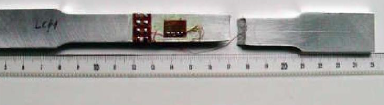
\includegraphics[scale=0.5]{figA0018.png}
  \end{center}
  \caption{Eprouvette d’aluminium après essai avec jauges de déformation.}
  \label{figA}
\end{figure}

\bigskip

On obtient les courbes contraintes-déformations suivantes.

\bigskip

\begin{minipage}{0.5\textwidth}
  %\begin{figure}
    \begin{center}
      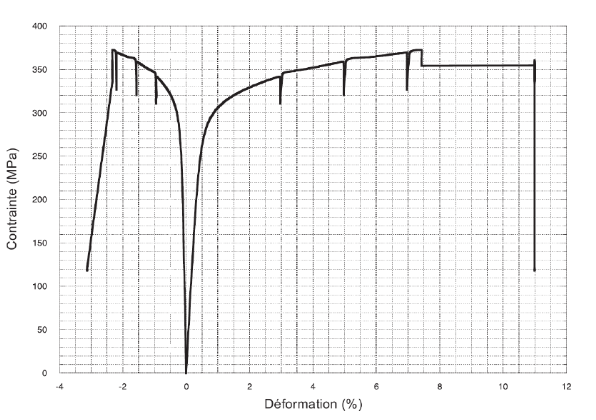
\includegraphics[width=\textwidth]{figB0018.png}
      \textbf{Courbe 1.}
    \end{center}
    %\caption{Courbe 1.}
    %\label{figB}
  %\end{figure}
\end{minipage}
\begin{minipage}{0.5\textwidth}
  %\begin{figure}
    \begin{center}
      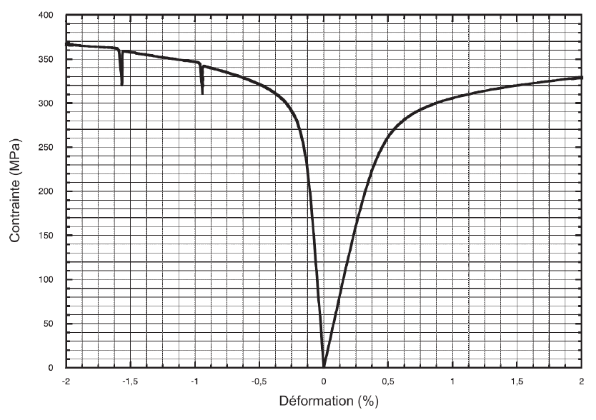
\includegraphics[width=\textwidth]{figC0018.png}
      \textbf{Courbe 2.}
    \end{center}
    %\caption{Courbe 2.}
    %\label{figC}
  %\end{figure}
\end{minipage}

\bigskip

\begin{enumerate}
  \item Identifier la courbe qui montre le comportement longitudinal, puis le comportement transversal. Justifier.
  \item Identifier sur les courbes la zone élastique et la zone plastique.
  \item Déterminer le module d'Young du matériau. Le comparer aux données du fournisseur qui sont
  $$72 \ GPa \ < \ E \ < \ 75,69 \ GPa$$
  \item Déterminer la contrainte limite d'élasticité du matériau $\sigma_{0}$ (appelée aussi $R_p$). La comparer aux données du fournisseur qui sont
  $$248  \ MPa \ < \ \sigma_{0} \ < \ 274,1 \ MPa$$
\end{enumerate}

\finenonce{rdm-0018}
\finexercice

\end{document}
